%  LaTeX support: latex@mdpi.com 
%  For support, please attach all files needed for compiling as well as the log file, and specify your operating system, LaTeX version, and LaTeX editor.

%=================================================================
\documentclass[journal,article,submit,pdftex,moreauthors]{Definitions/mdpi} 

\usepackage{longtable}
\usepackage{multirow}
\usepackage{booktabs}
\usepackage{adjustbox}
\usepackage{changepage}
\usepackage{tikz}

\usetikzlibrary{shapes.geometric, arrows}

%--------------------
% Class Options:
%--------------------
%----------
% journal
%----------
% Choose between the following MDPI journals:
% For posting an early version of this manuscript as a preprint, you may use "preprints" as the journal. Changing "submit" to "accept" before posting will remove line numbers.

%---------
% article
%---------
% The default type of manuscript is "article", but can be replaced by: 
% abstract, addendum, article, book, bookreview, briefreport, casereport, comment, commentary, communication, conferenceproceedings, correction, conferencereport, entry, expressionofconcern, extendedabstract, datadescriptor, editorial, essay, erratum, hypothesis, interestingimage, obituary, opinion, projectreport, reply, retraction, review, perspective, protocol, shortnote, studyprotocol, systematicreview, supfile, technicalnote, viewpoint, guidelines, registeredreport, tutorial
% supfile = supplementary materials

%----------
% submit
%----------
% The class option "submit" will be changed to "accept" by the Editorial Office when the paper is accepted. This will only make changes to the frontpage (e.g., the logo of the journal will get visible), the headings, and the copyright information. Also, line numbering will be removed. Journal info and pagination for accepted papers will also be assigned by the Editorial Office.

%------------------
% moreauthors
%------------------
% If there is only one author the class option oneauthor should be used. Otherwise use the class option moreauthors.

%---------
% pdftex
%---------
% The option pdftex is for use with pdfLaTeX. Remove "pdftex" for (1) compiling with LaTeX & dvi2pdf (if eps figures are used) or for (2) compiling with XeLaTeX.

%=================================================================
% MDPI internal commands - do not modify
\firstpage{1} 
\makeatletter 
\setcounter{page}{\@firstpage} 
\makeatother
\pubvolume{1}
\issuenum{1}
\articlenumber{0}
\pubyear{2024}
\copyrightyear{2024}
%\externaleditor{Academic Editor: Firstname Lastname}
\datereceived{ } 
\daterevised{ } % Comment out if no revised date
\dateaccepted{ } 
\datepublished{ } 
%\datecorrected{} % For corrected papers: "Corrected: XXX" date in the original paper.
%\dateretracted{} % For corrected papers: "Retracted: XXX" date in the original paper.
\hreflink{https://doi.org/} % If needed use \linebreak
%\doinum{}
%\pdfoutput=1 % Uncommented for upload to arXiv.org
%\CorrStatement{yes}  % For updates


%=================================================================
% Add packages and commands here. The following packages are loaded in our class file: fontenc, inputenc, calc, indentfirst, fancyhdr, graphicx, epstopdf, lastpage, ifthen, float, amsmath, amssymb, lineno, setspace, enumitem, mathpazo, booktabs, titlesec, etoolbox, tabto, xcolor, colortbl, soul, multirow, microtype, tikz, totcount, changepage, attrib, upgreek, array, tabularx, pbox, ragged2e, tocloft, marginnote, marginfix, enotez, amsthm, natbib, hyperref, cleveref, scrextend, url, geometry, newfloat, caption, draftwatermark, seqsplit
% cleveref: load \crefname definitions after \begin{document}

%=================================================================
% Please use the following mathematics environments: Theorem, Lemma, Corollary, Proposition, Characterization, Property, Problem, Example, ExamplesandDefinitions, Hypothesis, Remark, Definition, Notation, Assumption
%% For proofs, please use the proof environment (the amsthm package is loaded by the MDPI class).

%=================================================================
% Full title of the paper (Capitalized)
\Title{Analisis Faktor-Faktor Penentu Keberhasilan Implementasi Sistem Core Banking pada Lembaga Keuangan Mikro}

% MDPI internal command: Title for citation in the left column
\TitleCitation{Analisis Faktor-Faktor Penentu Keberhasilan Implementasi Sistem Core Banking pada Lembaa Keuangan Mikro}

% Author Orchid ID: enter ID or remove command
\newcommand{\orcidauthorA}{0000-0000-0000-000X} % Add \orcidA{} behind the author's name
%\newcommand{\orcidauthorB}{0000-0000-0000-000X} % Add \orcidB{} behind the author's name

% Authors, for the paper (add full first names)
% \Author{Firstname Lastname $^{1,\dagger,\ddagger}$\orcidA{}, Firstname Lastname $^{2,\ddagger}$ and Firstname Lastname $^{2,}$*}
\Author{Filzahanti Nuha Ramadhani$^{1,\ddagger}$, Samuel Mulatua Jeremy Nainggolan$^{1,\ddagger}$, Jon Felix Germinian$^{1,\ddagger}$}

%\longauthorlist{yes}

% MDPI internal command: Authors, for metadata in PDF
\AuthorNames{Firstname Lastname, Firstname Lastname and Firstname Lastname}

% MDPI internal command: Authors, for citation in the left column
\AuthorCitation{Lastname, F.; Lastname, F.; Lastname, F.}
% If this is a Chicago style journal: Lastname, Firstname, Firstname Lastname, and Firstname Lastname.

% Affiliations / Addresses (Add [1] after \address if there is only one affiliation.)
\address{%
$^{1}$ \quad Fakultas Ilmu Komputer Universitas Indonesia; filzahanti.nuha31@ui.ac.id\\
$^{2}$ \quad Fakultas Ilmu Komputer Universitas Indonesia; samuel.mulatua41@ui.ac.id\\
$^{3}$ \quad Fakultas Ilmu Komputer Universitas Indonesia; jon.felix@ui.ac.id\\
}

% Contact information of the corresponding author
% \corres{Correspondence: e-mail@e-mail.com; Tel.: (optional; include country code; if there are multiple corresponding authors, add author initials) +xx-xxxx-xxx-xxxx (F.L.)}

% Current address and/or shared authorship
\firstnote{Tugas Penelitian Sistem Informasi Perushaan}
\secondnote{These authors contributed equally to this work.}
% The commands \thirdnote{} till \eighthnote{} are available for further notes

%\simplesumm{} % Simple summary

%\conference{} % An extended version of a conference paper

% Abstract (Do not insert blank lines, i.e. \\) 
\abstract{Implementasi Core Banking System (CBS) merupakan langkah strategis untuk meningkatkan efisiensi operasional, keamanan, kualitas layanan, serta kepatuhan pada regulasi terkait penyelenggaraan teknologi informasi pada lembaga keuangan mikro, seperti Bank Perekonomian Rakyat (BPR). Namun kondisi yang ada menunjukan bahwa 45 persen BPR di Indonesia belum menerapkan CBS sesuai dengan amanat kewajiban utilisasi CBS menurut POJK SPTI tahun 2016, serta 30 persen implementasi CBS pada BPR di wilayah DKI Jaya gagal dilakukan sehingga penting bagi BPR yang belum menerapkan CBS untuk mempelajari faktor keberhasilan dari BPR yang telah sukses mengimplementasikan CBS guna mengakselerasi implementasi CBS pada organisasinya. Penelitian ini mengidentifikasi Critical Success Factors (CSF) untuk implementasi CBS dengan menggunakan kerangka People, Process, dan Technology. Data dikumpulkan dari pemimpin proyek implementasi CBS di sembilan BPR dan dianalisis menggunakan metode Fuzzy-AHP untuk menentukan peringkat CSF. Hasil penelitian menunjukkan bahwa dukungan manajemen senior, alokasi sumber daya, rekayasa ulang proses bisnis, kebutuhan sistem yang jelas, dan performa sistem adalah faktor yang paling berpengaruh. Temuan ini menekankan pentingnya strategi yang terarah untuk mengatasi hambatan implementasi CBS, terutama pada BPR dengan keterbatasan sumber daya. Penelitian ini memberikan kontribusi dengan menawarkan kerangka kerja praktis untuk mengoptimalkan adopsi CBS, meningkatkan kepatuhan terhadap standar regulasi, dan mendukung keberlanjutan operasional lembaga keuangan mikro.}

% Keywords
\keyword{Core Banking System; Critical Success Factors; Lembaga Keuangan Mikro; Fuzzy-AHP} 

% The fields PACS, MSC, and JEL may be left empty or commented out if not applicable
%\PACS{J0101}
%\MSC{}
%\JEL{}

%%%%%%%%%%%%%%%%%%%%%%%%%%%%%%%%%%%%%%%%%%
% Only for the journal Diversity
%\LSID{\url{http://}}

%%%%%%%%%%%%%%%%%%%%%%%%%%%%%%%%%%%%%%%%%%
% Only for the journal Applied Sciences
%\featuredapplication{Authors are encouraged to provide a concise description of the specific application or a potential application of the work. This section is not mandatory.}
%%%%%%%%%%%%%%%%%%%%%%%%%%%%%%%%%%%%%%%%%%

%%%%%%%%%%%%%%%%%%%%%%%%%%%%%%%%%%%%%%%%%%
% Only for the journal Data
%\dataset{DOI number or link to the deposited data set if the data set is published separately. If the data set shall be published as a supplement to this paper, this field will be filled by the journal editors. In this case, please submit the data set as a supplement.}
%\datasetlicense{License under which the data set is made available (CC0, CC-BY, CC-BY-SA, CC-BY-NC, etc.)}

%%%%%%%%%%%%%%%%%%%%%%%%%%%%%%%%%%%%%%%%%%
% Only for the journal Toxins
%\keycontribution{The breakthroughs or highlights of the manuscript. Authors can write one or two sentences to describe the most important part of the paper.}

%%%%%%%%%%%%%%%%%%%%%%%%%%%%%%%%%%%%%%%%%%
% Only for the journal Encyclopedia
%\encyclopediadef{For entry manuscripts only: please provide a brief overview of the entry title instead of an abstract.}

%%%%%%%%%%%%%%%%%%%%%%%%%%%%%%%%%%%%%%%%%%
% Only for the journal Advances in Respiratory Medicine and Smart Cities
%\addhighlights{yes}
%\renewcommand{\addhighlights}{%

%\noindent This is an obligatory section in “Advances in Respiratory Medicine'' and ``Smart Cities”, whose goal is to increase the discoverability and readability of the article via search engines and other scholars. Highlights should not be a copy of the abstract, but a simple text allowing the reader to quickly and simplified find out what the article is about and what can be cited from it. Each of these parts should be devoted up to 2~bullet points.\vspace{3pt}\\
%\textbf{What are the main findings?}
% \begin{itemize}[labelsep=2.5mm,topsep=-3pt]
% \item First bullet.
% \item Second bullet.
% \end{itemize}\vspace{3pt}
%\textbf{What is the implication of the main finding?}
% \begin{itemize}[labelsep=2.5mm,topsep=-3pt]
% \item First bullet.
% \item Second bullet.
% \end{itemize}
%}

%%%%%%%%%%%%%%%%%%%%%%%%%%%%%%%%%%%%%%%%%%
\begin{document}

%%%%%%%%%%%%%%%%%%%%%%%%%%%%%%%%%%%%%%%%%%
% \setcounter{section}{-1} %% Remove this when starting to work on the template.
% \section{How to Use this Template}

% The template details the sections that can be used in a manuscript. Note that the order and names of article sections may differ from the requirements of the journal (e.g., the positioning of the Materials and Methods section). Please check the instructions on the authors' page of the journal to verify the correct order and names. For any questions, please contact the editorial office of the journal or support@mdpi.com. For LaTeX-related questions please contact latex@mdpi.com.%\endnote{This is an endnote.} % To use endnotes, please un-comment \printendnotes below (before References). Only journal Laws uses \footnote.

% The order of the section titles is different for some journals. Please refer to the "Instructions for Authors” on the journal homepage.

\section{Pendahuluan}

\subsection{Latar Belakang}

Dalam beberapa tahun terakhir, lembaga keuangan mikro seperti Bank Perekonomian Rakyat (BPR) dan Koperasi Simpan Pinjam (KSP) telah mengalami pertumbuhan pesat di Indonesia \cite{OJK2024roadmap}. Lembaga-lembaga ini memainkan peran penting dalam inklusi keuangan, terutama bagi masyarakat yang belum terjangkau oleh perbankan konvensional. Namun, seiring dengan pertumbuhan tersebut, tantangan dalam efisiensi pengelolaan data, keamanan transaksi, dan kecepatan pelayanan menjadi semakin kompleks. Untuk mengatasi hal ini, adopsi teknologi informasi, khususnya aplikasi inti perbankan atau core banking system (CBS), menjadi solusi strategis. CBS memungkinkan pengelolaan berbagai aspek operasional secara terintegrasi, seperti manajemen simpanan, pinjaman, hingga pelaporan keuangan dan kepatuhan terhadap regulasi dari otoritas seperti Bank Indonesia (BI) dan Otoritas Jasa Keuangan (OJK).

POJK 75/POJK.03/2016 tentang Standar Penyelenggaraan Teknologi Informasi BPR menyatakan bahwa setiap BPR wajib menggunakan CBS yang memenuhi persyaratan yang ditetapkan. Meski demikian, implementasi CBS di BPR menghadapi tantangan yang signifikan. Hasil wawancara dengan Ketua Perbarindo DKI Jakarta menunjukkan bahwa dalam lima tahun terakhir, sebanyak 30 persen implementasi CBS di BPR wilayah DKI Jaya mengalami kegagalan. Data dari penelitian OJK dan ILO  \cite{Sitorus2023digital} juga mengungkapkan bahwa 45 persen BPR di Indonesia masih belum sepenuhnya menerapkan CBS sesuai dengan ketentuan dalam POJK. Keterlambatan ini dipengaruhi oleh beragam faktor, termasuk perbedaan kapasitas modal, kesiapan infrastruktur, dan kemampuan organisasi untuk beradaptasi dengan teknologi baru.

Dalam Roadmap Pengembangan dan Penguatan Industri BPR dan BPRS (RP2B) 2024-2027 \cite{OJK2024roadmap}, disebutkan bahwa transformasi digital melalui implementasi CBS adalah salah satu prioritas utama untuk meningkatkan daya saing BPR/BPRS, terutama di tengah persaingan dengan bank umum dan perusahaan teknologi finansial (fintech) serta ketertinggalan implementasi dari regulasi yan telah ditetapkan sebelumnya. Dalam hal ini penting bagi BPR yang belum menerapkan CBS untuk mempelajari faktor-faktor keberhasilan dari BPR yang telah sukses mengimplementasikan teknologi ini. Dengan memahami praktik terbaik dan strategi yang diterapkan oleh BPR yang berhasil, diharapkan percepatan implementasi CBS di seluruh BPR dapat tercapai, sehingga lembaga-lembaga ini dapat memanfaatkan teknologi untuk meningkatkan efisiensi, keamanan, dan pelayanan terhadap nasabah. Penelitian ini bertujuan untuk mengidentifikasi faktor-faktor yang menentukan kesuksesan implementasi CBS, dengan mengambil studi kasus pada klien-klien PT Dimensi Kreasi Nusantara. Kajian ini juga akan mengeksplorasi hambatan dan kesiapan implementasi CBS berdasarkan perbedaan skala aset dan kondisi operasional BPR. Dengan demikian, penelitian ini diharapkan dapat memberikan panduan strategis bagi BPR untuk mengoptimalkan transformasi digitalnya melalui CBS.

\subsection{Perumusan Masalah}

Penelitian ini bertujuan untuk mengeksplorasi faktor-faktor yang mempengaruhi keberhasilan implementasi \textit{core banking system} di lembaga keuangan mikro, menggunakan kerangka \textit{People}, \textit{Process}, dan \textit{Technology}. \textit{Core banking system} menjadi solusi strategis bagi lembaga keuangan mikro dalam meningkatkan efisiensi, keamanan, dan kecepatan pelayanan. Namun, adopsi teknologi ini menghadapi tantangan yang bervariasi tergantung pada ukuran aset, jumlah rekening, dan kompleksitas operasional. Oleh karena itu, penelitian ini akan mengkaji secara mendalam faktor-faktor yang berkontribusi terhadap keberhasilan implementasi sistem ini di berbagai kategori lembaga keuangan mikro

Dari perspektif \textit{People}, penelitian ini akan fokus pada bagaimana dukungan manajemen mempengaruhi keberhasilan implementasi \textit{core banking system}. Selain itu, aspek adaptasi teknologi oleh karyawan juga menjadi kunci penting yang akan diteliti, terutama dalam hal kesiapan sumber daya manusia dalam menerima perubahan teknologi. Perbedaan dalam tingkat kesiapan sumber daya manusia di lembaga keuangan mikro dengan aset besar dan kecil juga akan dianalisis untuk melihat dampaknya terhadap proses adopsi teknologi.

Dalam aspek \textit{Process}, penelitian ini akan mengeksplorasi bagaimana proses bisnis yang ada di lembaga keuangan mikro berdampak pada implementasi \textit{core banking system}. Kompleksitas operasional juga menjadi fokus, mengingat bahwa lembaga dengan struktur operasional yang lebih rumit mungkin menghadapi tantangan yang lebih besar dalam mengintegrasikan sistem baru. Penelitian ini juga akan mengeksplorasi bagaimana lembaga keuangan mikro mengelola perubahan proses kerja yang diperlukan untuk memaksimalkan manfaat dari \textit{core banking system}.

Dari sisi \textit{Technology}, penelitian ini akan mengidentifikasi tantangan yang berkaitan dengan infrastruktur teknologi yang digunakan oleh lembaga keuangan mikro. Ketersediaan teknologi yang memadai menjadi faktor penting dalam memastikan kelancaran implementasi dan operasional \textit{core banking system}. Selain itu, penelitian ini juga akan membandingkan kemampuan lembaga dengan kapasitas teknologi yang berbeda dalam mengadopsi dan memanfaatkan \textit{core banking system} secara efektif, terutama dalam konteks lembaga yang memiliki sumber daya teknologi terbatas

Dengan demikian pertanyaan yang diangkat di penelitian ini adalah sebagai berikut:
\begin{itemize}
    \item Apa saja faktor kunci yang menentukan keberhasilan implementasi \textit{core banking system} pada lembaga keuangan mikro?
\end{itemize}

\subsection{Tujuan Penelitian}
Tujuan dari penelitian ini adalah untuk mengidentifikasi urutan faktor kunci utama kesuksesan dalam implementasi \textit{core banking system} di lembaga keuangan mikro.

\subsection{Manfaat Penelitian}
Penelitian ini dapat memberikan wawasan mengenai urutan faktor-faktor kunci yang menentukan keberhasilan implementasi \textit{core banking system}, sehingga dapat membantu lembaga keuangan mikro dalam memprioritaskan solusi yang sesuai dengan memahami faktor-faktor yang paling berpengaruh terhadap keberhasilan implementasi \textit{core banking system} dan menjalankan proyek implementasi teknologi \textit{core banking system} yang lebih efektif. Dengan memahami tantangan dan kebutuhan spesifik, lembaga keuangan dapat memaksimalkan efisiensi, produktivitas, dan pelayanan kepada nasabah.

% -------------------------------------------------------------------------------------------------------------------------------------------------


\section{Studi Literatur} \label{sec:Studi Literatrur}

Bagian ini menjelaskan tentang landasan teori yang digunakan dalam melakukan penelitian, yaitu mengenai \textit{core banking system} dan \textit{critical success factor}. Selain itu pada bab ini akan dibahas mengenai kajian dari hasil - hasil penelitian sebelumnya yang terkait dengan penelitian ini.

\subsection{Core Banking System} \label{sec:Core Banking System}

\textit{Core Banking System} (CBS) adalah sistem informasi terpusat yang memungkinkan bank memproses dan mengelola berbagai transaksi finansial dan layanan perbankan secara real-time. CBS mencakup fungsi-fungsi dasar perbankan seperti transfer dana, pengelolaan akun, deposito, dan peminjaman. Sistem ini diakses oleh cabang-cabang bank dan platform digital secara langsung, sehingga menciptakan efisiensi dan konsistensi layanan perbankan. CBS merupakan "jantung" operasional bank yang mengotomatisasi sebagian besar proses internal dan eksternal untuk memastikan kelancaran transaksi harian serta pengelolaan data nasabah dengan aman dan cepat \cite{Hsiao-ebanking}.


CBS memberikan banyak manfaat bagi institusi perbankan, termasuk efisiensi operasional yang lebih tinggi, integrasi data yang lebih baik, serta peningkatan pengalaman nasabah. Kualitas sistem dan informasi yang baik dapat meningkatkan kepuasan pengguna internal dan eksternal. Di PT Bank Perkreditan Rakyat (BPR) Hasamitra, kualitas sistem dan manfaat sistem CBS terbukti berpengaruh positif terhadap kinerja bank, termasuk penyediaan layanan yang lebih cepat dan andal \cite{basyir-cbs}. CBS juga memfasilitasi pengambilan keputusan yang lebih baik melalui integrasi data yang efektif, yang pada gilirannya meningkatkan daya saing bank di pasar \cite{pratama-cbs}.


Meskipun CBS menawarkan berbagai manfaat, implementasi sistem ini dihadapkan pada sejumlah tantangan, terutama dalam hal adaptasi teknologi dan manajemen perubahan. Di Vietnam, penelitian menunjukkan bahwa kualitas layanan menjadi tantangan terbesar dalam memastikan kepuasan pengguna CBS, yang sering kali terhambat oleh ketergantungan pada infrastruktur teknologi yang ketinggalan zaman \cite{Hsiao-ebanking}. Selain itu, audit sistem CBS menggunakan ITIL menggarisbawahi perlunya pengelolaan siklus hidup layanan yang tepat untuk menghindari kegagalan operasional dan memastikan keberlanjutan sistem dalam jangka panjang \cite{wahyudi-cbs}. Implementasi CBS juga memerlukan penyesuaian budaya organisasi dan pelatihan intensif bagi karyawan untuk mengoptimalkan penggunaannya.

\subsection{Critical Success Factors}
    \textit{Critical Success Factors} (CSF) pada sistem informasi merujuk pada elemen-elemen kunci yang menentukan keberhasilan implementasi dan operasionalisasi suatu sistem informasi. CSF mencakup berbagai aspek yang harus diperhatikan secara cermat, termasuk faktor organisasi, teknis, dan pengguna. Dalam implementasi sistem informasi bisnis seperti \textit{Business Intelligence} (BI), CSF meliputi pemberdayaan organisasi, kemudahan penggunaan sistem, dan dukungan pengguna yang tepat \cite{harfoush2024critical}. Pada sistem DevOps, faktor kolaborasi, praktik teknis, dan pengukuran juga sangat krusial untuk memastikan kelancaran pengembangan perangkat lunak \cite{jayakody2023devops}. Sementara itu, dalam sistem informasi rumah sakit, CSF meliputi keandalan, kemudahan penggunaan, dan kecocokan organisasi yang berpengaruh besar terhadap keberhasilan sistem \cite{arpaci2023hospital}. Dalam sistem perbankan akan didiskusikan lebih lanjut pada subbab \ref{sec:Penelitian Terdahulu} 

\subsubsection{Manfaat Identifikasi \textit{Critical Success Factors} (CSF)}
Mengidentifikasi dan memahami CSF dalam pengembangan sistem informasi memberikan berbagai manfaat penting. CSF membantu organisasi memastikan bahwa faktor-faktor utama yang mempengaruhi keberhasilan proyek sistem informasi dikelola dengan baik sejak awal. Dalam sistem informasi kesehatan, penerapan dan manajemen CSF secara prospektif dapat membantu dalam adaptasi situasional dan mengurangi risiko kegagalan sistem \cite{aggestam2023apply}. Lebih jauh lagi, pemahaman yang jelas tentang CSF memungkinkan organisasi untuk mengalokasikan sumber daya secara efektif, meningkatkan kepuasan pengguna, dan memastikan sistem tetap relevan dengan kebutuhan operasional dan teknologi yang berubah-ubah. Studi-studi menunjukkan bahwa pengelolaan CSF yang baik dapat mempercepat proses adopsi teknologi, meningkatkan produktivitas, dan mengurangi hambatan dalam pengembangan sistem informasi \cite{jayakody2023devops}.

\subsection{Analytic Hierarchy Process (AHP)}

Analytic Hierarchy Process (AHP) adalah metode pengambilan keputusan yang dikembangkan oleh Thomas Saaty pada tahun 1980 \cite{Saaty}, digunakan untuk menyelesaikan masalah kompleks dengan berbagai kriteria. AHP menyusun masalah dalam struktur hierarki, dengan tujuan utama di bagian atas dan kriteria di bawahnya, kemudian mengevaluasi dan menentukan prioritas elemen-elemen tersebut melalui tiga langkah utama: konstruksi hierarki, analisis prioritas dengan perbandingan berpasangan, dan verifikasi konsistensi. Meskipun memberikan pendekatan terstruktur untuk pengambilan keputusan yang jelas dan konsisten, AHP memiliki kelemahan dalam menangani informasi yang tidak pasti atau ambigu, karena metode ini mengandalkan perbandingan pasti yang mungkin tidak dapat diterapkan dengan baik pada situasi dengan data yang tidak lengkap atau subjektif \cite{fahpbook}.


\subsection{Fuzzy Analytic Hierarchy Process (Fuzzy-AHP)}

Fuzzy-AHP adalah pengembangan dari AHP tradisional yang mengatasi data yang tidak tepat atau kabur dengan menggunakan logika fuzzy. Alih-alih bergantung pada angka yang pasti, Fuzzy-AHP menggunakan angka fuzzy untuk mewakili penilaian yang kabur sehingga memungkinkan pengambil keputusan untuk menyatakan preferensi mereka dengan istilah seperti "sedikit lebih penting" atau "jauh lebih penting." Fuzzy-AHP membantu mengelola ketidakpastian dalam pengambilan keputusan dengan memberikan derajat keanggotaan (\textit{membership degrees}) pada angka fuzzy tersebut \cite{liu-fahp}.

Proses membangun model Fuzzy-AHP meliputi pembuatan matriks perbandingan, menggabungkan berbagai penilaian, memeriksa konsistensi, dan mengubah bobot fuzzy menjadi nilai pasti (defuzzifikasi). Namun, penggunaan himpunan fuzzy membuat perhitungan lebih kompleks karena metode tradisional seperti eigenvektor dan rata-rata geometrik tidak dapat diterapkan langsung pada matriks perbandingan fuzzy. Walaupun demikian, Fuzzy-AHP sangat berguna dalam situasi dunia nyata di mana data tidak jelas atau tidak pasti dengan memberikan pendekatan yang fleksibel untuk pengambilan keputusan \cite{liu-fahp}.

\subsection{Penelitian Terdahulu} \label{sec:Penelitian Terdahulu}

Studi mengenai \textit{critical success factors} (CSF) dalam implementasi sistem informasi \textit{Core Banking System} (CBS) menyoroti pentingnya dukungan manajemen puncak, metode manajemen proyek yang tepat, dan pelatihan pengguna akhir. Penelitian oleh Ghafari, H \cite{Ghafari-csf} menemukan bahwa faktor-faktor utama yang berpengaruh dalam keberhasilan implementasi CBS di Bank of Industry and Mine mencakup dukungan manajemen senior, rekayasa ulang proses bisnis, dan dukungan vendor. Dari faktor-faktor tersebut, dukungan manajemen senior dan pelatihan pengguna akhir memberikan dampak terbesar terhadap keberhasilan implementasi CBS.

Selain itu, penelitian di Nigeria menunjukkan bahwa manajemen risiko sistem informasi juga memainkan peran penting dalam keberhasilan CBS, terutama dalam mengatasi ancaman dan ketidakpastian yang terkait dengan informasi. Dukungan manajemen puncak, struktur organisasi, dan alokasi sumber daya yang memadai adalah kunci utama keberhasilan manajemen risiko sistem informasi di sektor perbankan Nigeria, yang pada akhirnya berkontribusi terhadap peningkatan kinerja bank \cite{falisat-csf}.

Studi lain \cite{salu-csf} di sektor perbankan India menyoroti sepuluh faktor sukses utama dalam adopsi CBS, seperti kompatibilitas, kompleksitas, dukungan manajemen, infrastruktur, keamanan, dan kebijakan pemerintah. Dengan menggunakan model struktural interpretatif, penelitian ini mengidentifikasi hubungan antara variabel-variabel tersebut dan menekankan pentingnya dukungan manajemen serta kesadaran akan keamanan sebagai faktor kunci adopsi CBS \cite{salu-csf}.

Kesuksesan implementasi CBS juga dipengaruhi oleh kesiapan organisasi dalam mengelola perubahan \cite{johny-csf}. Studi ini menemukan bahwa implementasi CBS yang efektif memerlukan pemahaman mendalam tentang proses implementasi, tantangan teknis, serta kesiapan teknologi dan tenaga kerja. Kurangnya pelatihan dan keterampilan teknis dapat menyebabkan kegagalan implementasi sistem CBS yang kompleks \cite{johny-csf}.

Kajla et al. (2021) mengkaji faktor-faktor kritis yang mempengaruhi adopsi \textit{blockchain} di sektor perbankan dengan menggunakan kerangka kerja Technology-Organization-Environment (TOE) dan Fuzzy Analytic Hierarchy Process (Fuzzy-AHP). Meskipun fokus penelitian ini adalah adopsi blockchain, metode Fuzzy-AHP yang digunakan juga relevan dengan penelitian tentang implementasi CBS. Penulis menggunakan Fuzzy-AHP dalam penelitian mereka karena memungkinkan integrasi pendapat ahli \cite{KajlaFAHP}. Penelitian lain menggunakan FAHP untuk memprioritaskan faktor-faktor kunci keberhasilan (CSF) pada proyek TI di sektor perbankan, asuransi, dan ritel. FAHP digunakan karena memungkinkan penilaian yang fleksibel dengan menggunakan nilai interval. Dengan mengintegrasikan logika fuzzy dalam pengambilan keputusan multi-kriteria, FAHP memberikan kerangka kerja yang lebih terstruktur untuk memprioritaskan faktor-faktor yang mempengaruhi keberhasilan proyek TI \cite{Siddique-fahp}.

% -------------------------------------------------------------------------------------------------------------------------------------------------

\section{Metodologi}
Penelitian ini menggunakan pendekatan kuantitatif dengan menggunakan data yang dikumpulkan dari kuesioner yang dirancang berdasarkan hierarki CSF implementasi CBS. Terdapat 19 responden, 2 responden merupakan karyawan System Implementor CBS di PT DKN, dan 17 lainnya merupakan orang yang bertanggung jawab atas implementasi CBS dari 9 BPR dengan jabatan sebagai Pejabat Eksekutif (PE) atau Direksi. Kemudian responden diminta untuk meninjau dan mengisi kuesioner yang berisi faktor-faktor keberhasilan implementasi \textit{core banking system}. Setelah responden mengisi kuesioner yang diberikan, urutan dari faktor-faktor kesuksesan dicari menggunakan Fuzzy-AHP. CSF harus diidentifikasi untuk mengurangi tingkat kegagalan implementasi \textit{core banking system} \cite{aggestam2023apply}. Figure \ref{fig:tahapan} di bawah merupakan ringkasan dari tahapan penelitian.

% \begin{figure}[H]
% \includegraphics[width=6 cm]{attachments/tahapan.png}
% \caption{Tahapan Penelitian \label{fig:tahapan}}
% \end{figure}   

\begin{figure}[H]
    \centering
    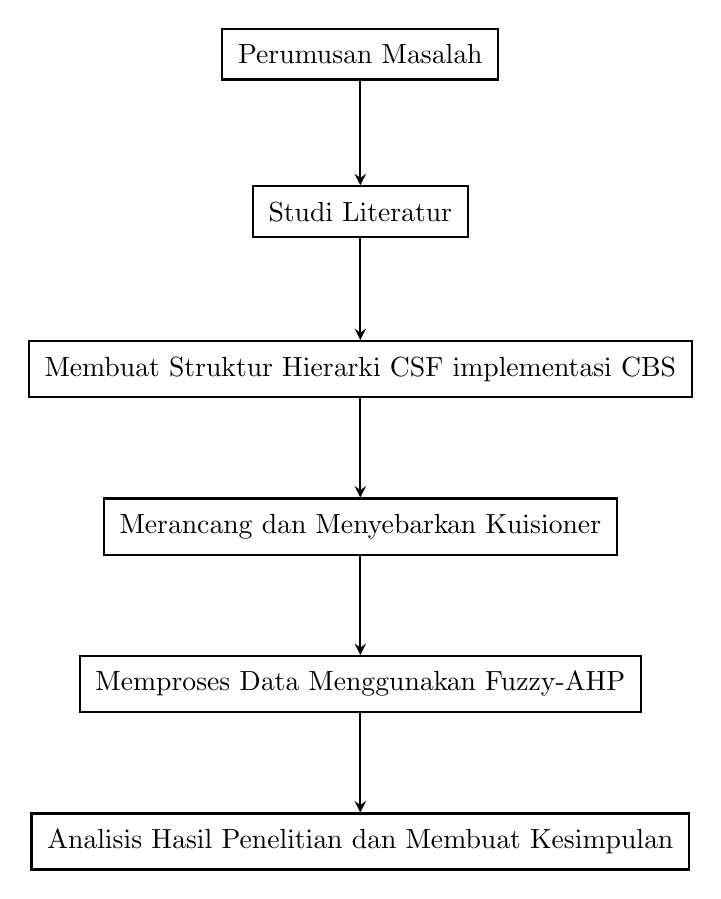
\begin{tikzpicture}[node distance=2cm]
        \tikzstyle{step} = [rectangle, rounded corners, minimum width=3cm, minimum height=1cm,text centered, draw=black, fill=lightgray]
        \tikzstyle{arrow} = [thick,->,>=stealth]
        \tikzstyle{box} = [draw=black, thick, inner sep=0.2cm]
        
        % Nodes
        \node (problem) [box] {Perumusan Masalah};
        \node (literature) [box, below of=problem] {Studi Literatur};
        \node (hierarchy) [box, below of=literature] {Membuat Struktur Hierarki CSF implementasi CBS};
        \node (questionnaire) [box, below of=hierarchy] {Merancang dan Menyebarkan Kuisioner};
        \node (processing) [box, below of=questionnaire] {Memproses Data Menggunakan Fuzzy-AHP};
        \node (analysis) [box, below of=processing] {Analisis Hasil Penelitian dan Membuat Kesimpulan};

        % Arrows
        \draw [arrow] (problem) -- (literature);
        \draw [arrow] (literature) -- (hierarchy);
        \draw [arrow] (hierarchy) -- (questionnaire);
        \draw [arrow] (questionnaire) -- (processing);
        \draw [arrow] (processing) -- (analysis);

    \end{tikzpicture}
    \caption{Langkah-langkah Penelitian}
     \label{fig:tahapan}}
\end{figure}

% People
% - Dukungan manajemen senior \cite{Ghafari-csf} \cite{falisat-csf} 
% - Alokasi sumber daya \cite{falisat-csf} 
% - Kompatibilitas Teknologi \cite{salu-csf} \cite{johny-csf}
% - Perubahan manajemen dan Adaptasi User \cite{Ghafari-csf}

% Process
% - Rekayasa ulang proses bisnis \cite{falisat-csf}
% - Kebutuhan sistem yang jelas \cite{johny-csf}
% - Standar operasional yang jelas \cite{salu-csf}
% - Mitigasi and manajemen resiko \cite{falisat-csf}

% Teknologi
% - Keamanan yang kuat \cite{falisat-csf}
% - Skalabilitas infrastruktur IT \cite{Ghafari-csf} \cite{salu-csf}
% - Integrasi Sistem \cite{Ghafari-csf}
% - Performa dan kecepatan sistem \cite{Ghafari-csf}

\subsection{Critical Success Factor CBS}


\textit{Critical Success Factors} (CSF) sistem core banking diidentifikasi melalui tinjauan pustaka dari jurnal sistem informasi berkualitas tinggi yang diterbitkan antara tahun 2016 dan 2024 \cite{Ghafari-csf} \cite{falisat-csf} \cite{salu-csf} \cite{johny-csf}. Tinjauan ini difokuskan pada database seperti IEEE Xplore, ScienceDirect, dan ProQuest. Kata kunci yang digunakan untuk pencarian pustaka mencakup "\textit{critical success factors}", “\textit{success factors}”, "\textit{core banking system}", "\textit{banking system}", dan beberapa lainnya. CSF yang diteliti dapat dilihat pada tabel \ref{csf-table}


\begin{table}[h!]
\begin{adjustwidth}{-\extralength}{0cm}
    \caption{Critical Success Factors (CSFs) dalam Implementasi Sistem Informasi}
    \label{csf-table}
    \centering
    \begin{tabular}{c|c|p{4cm}|p{6cm}|c}
        \toprule
        \textbf{Context} & \textbf{CSF Code} & \textbf{Critical Success Factors} & \textbf{Penjelasan Singkat} & \textbf{Reference} \\ 
        \midrule
        \textbf{People} & PP1 & \raggedright Dukungan manajemen senior & \raggedright Keterlibatan manajemen senior sangat penting dalam alokasi sumber daya dan arah proyek. & \cite{Ghafari-csf}, \cite{falisat-csf} \\ 
        \midrule
        \textbf{People} & PP2 & \raggedright Alokasi sumber daya & \raggedright Sumber daya yang memadai diperlukan untuk keberhasilan implementasi sistem. & \cite{falisat-csf} \\ 
        \midrule
        \textbf{People} & PP3 & \raggedright Kompatibilitas Teknologi & \raggedright Teknologi yang kompatibel dengan infrastruktur yang ada sangat penting untuk integrasi yang lancar. & \cite{salu-csf}, \cite{johny-csf} \\ 
        \midrule
        \textbf{People} & PP4 & \raggedright Perubahan manajemen dan Adaptasi User & \raggedright Manajemen perubahan yang baik membantu pengguna beradaptasi dengan sistem baru. & \cite{Ghafari-csf} \\ 
        \midrule
        \textbf{Process} & PR1 & \raggedright Rekayasa ulang proses bisnis & \raggedright Proses bisnis perlu direkayasa ulang untuk mendukung implementasi sistem yang lebih efisien. & \cite{falisat-csf} \\ 
        \midrule
        \textbf{Process} & PR2 & \raggedright Kebutuhan sistem yang jelas & \raggedright Kebutuhan sistem yang jelas membantu memastikan kesuksesan implementasi. & \cite{johny-csf} \\ 
        \midrule
        \textbf{Process} & PR3 & \raggedright Standar operasional yang jelas & \raggedright Standar operasional diperlukan untuk menjaga konsistensi dan efisiensi. & \cite{salu-csf} \\ 
        \midrule
        \textbf{Process} & PR4 & \raggedright Mitigasi dan manajemen risiko & \raggedright Penting untuk mengidentifikasi dan mengelola risiko untuk mencegah kegagalan sistem. & \cite{falisat-csf} \\ 
        \midrule
        \textbf{Teknologi} & TT1 & \raggedright Keamanan yang kuat & \raggedright Keamanan data adalah prioritas utama untuk melindungi informasi sensitif. & \cite{falisat-csf} \\ 
        \midrule
        \textbf{Teknologi} & TT2 & \raggedright Skalabilitas infrastruktur IT & \raggedright Infrastruktur IT harus dapat diskalakan untuk mendukung pertumbuhan masa depan. & \cite{Ghafari-csf}, \cite{salu-csf} \\ 
        \midrule
        \textbf{Teknologi} & TT3 & \raggedright Integrasi Sistem & \raggedright Sistem baru harus terintegrasi dengan lancar dengan sistem yang ada. & \cite{Ghafari-csf} \\ 
        \midrule
        \textbf{Teknologi} & TT4 & \raggedright Performa dan kecepatan sistem & \raggedright Performa sistem yang cepat meningkatkan efisiensi operasional dan kepuasan pengguna. & \cite{Ghafari-csf} \\ 
        \bottomrule
    \end{tabular}
\end{adjustwidth}
\end{table}

% \begin{longtable}{c|c|p{4cm}|p{6cm}|c}

%     \caption{Critical Success Factors (CSFs) dalam Implementasi Sistem Informasi} \label{csf-table} \\
%     \hline
%     \textbf{Context} & \textbf{CSF Code} & \textbf{Critical Success Factors} & \textbf{Penjelasan Singkat} & \textbf{Reference} \\
%     \hline
%     \endfirsthead
%     % Head for the first page
%     \multicolumn{5}{c}{\textit{Lanjutan dari halaman sebelumnya}} \\
%     \hline
%     \textbf{Context} & \textbf{CSF Code} & \textbf{Critical Success Factors} & \textbf{Penjelasan Singkat} & \textbf{Reference} \\
%     \hline
%     \endhead
%     % Head for subsequent pages
%     \hline
%     \multicolumn{5}{|r|}{\textit{Lanjut ke halaman berikutnya}} \\
%     \hline
%     \endfoot
%     % Foot for all pages
%     \hline
%     \endlastfoot
%     % Foot for the last page
%     \begin{adjustwidth}{-\extralength}{0cm}
%     \textbf{People} & PP1 & \raggedright Dukungan manajemen senior & \raggedright Keterlibatan manajemen senior sangat penting dalam alokasi sumber daya dan arah proyek. & \cite{Ghafari-csf}, \cite{falisat-csf} \\ 
%     \hline
%     \textbf{People} & PP2 & \raggedright Alokasi sumber daya & \raggedright Sumber daya yang memadai diperlukan untuk keberhasilan implementasi sistem. & \cite{falisat-csf} \\ 
%     \hline
%     \textbf{People} & PP3 & \raggedright Kompatibilitas Teknologi & \raggedright Teknologi yang kompatibel dengan infrastruktur yang ada sangat penting untuk integrasi yang lancar. & \cite{salu-csf}, \cite{johny-csf} \\ 
%     \hline
%     \textbf{People} & PP4 & \raggedright Perubahan manajemen dan Adaptasi User & \raggedright Manajemen perubahan yang baik membantu pengguna beradaptasi dengan sistem baru. & \cite{Ghafari-csf} \\ 
%     \hline
%     \textbf{Process} & PR1 & \raggedright Rekayasa ulang proses bisnis & \raggedright Proses bisnis perlu direkayasa ulang untuk mendukung implementasi sistem yang lebih efisien. & \cite{falisat-csf} \\ 
%     \hline
%     \textbf{Process} & PR2 & \raggedright Kebutuhan sistem yang jelas & \raggedright Kebutuhan sistem yang jelas membantu memastikan kesuksesan implementasi. & \cite{johny-csf} \\ 
%     \hline
%     \textbf{Process} & PR3 & \raggedright Standar operasional yang jelas & \raggedright Standar operasional diperlukan untuk menjaga konsistensi dan efisiensi. & \cite{salu-csf} \\ 
%     \hline
%     \textbf{Process} & PR4 & \raggedright Mitigasi dan manajemen risiko & \raggedright Penting untuk mengidentifikasi dan mengelola risiko untuk mencegah kegagalan sistem. & \cite{falisat-csf} \\ 
%     \hline
%     \textbf{Teknologi} & TT1 & \raggedright Keamanan yang kuat & \raggedright Keamanan data adalah prioritas utama untuk melindungi informasi sensitif. & \cite{falisat-csf} \\ 
%     \hline
%     \textbf{Teknologi} & TT2 & \raggedright Skalabilitas infrastruktur IT & \raggedright Infrastruktur IT harus dapat diskalakan untuk mendukung pertumbuhan masa depan. & \cite{Ghafari-csf}, \cite{salu-csf} \\ 
%     \hline
%     \textbf{Teknologi} & TT3 & \raggedright Integrasi Sistem & \raggedright Sistem baru harus terintegrasi dengan lancar dengan sistem yang ada. & \cite{Ghafari-csf} \\ 
%     \hline
%     \textbf{Teknologi} & TT4 & \raggedright Performa dan kecepatan sistem & \raggedright Performa sistem yang cepat meningkatkan efisiensi operasional dan kepuasan pengguna. & \cite{Ghafari-csf} \\ 
%     \end{adjustwidth}
% \end{longtable}

\subsection{Sample dan Populasi}
Populasi dalam penelitian ini adalah Bank Perkreditan Rakyat (BPR) yang telah berhasil mengimplementasikan Core Banking System. Sampel yang diambil merupakan representasi karyawan dari masing-masing kelompok usaha BPR.

\subsection{Instrumen}
Instrumen dalam penelitian ini adalah kuisioner yang terdiri dari lima bagian. Bagian pertama dari survei berisi data pribadi responden. Bagian kedua berisi komparasi terhadap kriteria People, Process, dan Technology. Bagian-bagian selanjutnya berisi komparasi masing-masing Critical Success Factor (CSF) dari People, Process, dan Technology. Skala yang digunakan adalah skala Linguistik, yang dapat dilihat pada Tabel \ref{tab:fuzzy-segitiga}.

\subsection{Pengumpulan Data}
Distribusi kuisioner dilakukan menggunakan platform Formbricks dengan tautan \url{https://app.formbricks.com/s/cm3bidub8000afrf8qw41o4fh}. Tautan ini diberikan secara individu kepada setiap responden. Survei dilaksanakan mulai dari 11 November 2024 hingga 1 Desember 2024.


\subsection{Fuzzy Analytical Hierarchy Process (Fuzzy-AHP)}

Fuzzy-AHP merupakan pengembangan dari metode AHP \cite{Saaty}. Dalam penelitian ini, Fuzzy-AHP yang digunakan mengacu pada metode yang dikembangkan oleh Buckley pada tahun 1985 \cite{buckley-fahp}. Metode ini menggunakan bilangan fuzzy segitiga untuk skala perbandingan berpasangan dalam Fuzzy AHP untuk menggantikan bilangan pasti pada skala Saaty. Metode ini mengatasi ketidakpastian yang sering kali muncul dalam masalah pengambilan keputusan dunia nyata dan memungkinkan pengambilan keputusan berdasarkan penilaian subjektif yang lebih fleksibel. Saat ini, Fuzzy-AHP juga banyak digunakan di berbagai bidang seperti bisnis, manajemen, manufaktur, industri, dan pemerintahan \cite{fahpbook}.

\begin{table}[H]
    \caption{Bilangan Fuzzy Segitiga yang Digunakan}
    \label{tab:fuzzy-segitiga}
    \centering
    \begin{tabular}{c|c|c}
        \toprule
        \textbf{Skala Linguistik} & \textbf{Bilangan Fuzzy Segitiga} & \textbf{Bilangan Fuzzy Segitiga Resiprokal}\\ 
        \midrule
        \raggedright Mutlak Lebih Penting & (9,9,9) & (1/9,1/9,1/9) \\ 
        \midrule
        \raggedright Sangat Lebih Penting & (6,7,8) & (1/8,1/7,1/6) \\ 
        \midrule
        \raggedright Cukup Lebih Penting & (4,5,6) & (1/6,1/5,1/4) \\ 
        \midrule
        \raggedright Sedikit Lebih Penting & (2,3,4) & (1/4,1/3,1/2) \\ 
        \midrule
        \raggedright Sama Pentingnya & (1,1,1) & (1,1,1) \\ 
        \bottomrule
    \end{tabular}
\end{table}


Penjelasan detail mengenai tahapan-tahapan perhitungan metode Fuzzy-AHP akan diuraikan sebagai berikut.

Pada tahap perbandingan, penelitian ini menggunakan metode \textit{pairwise comparison}. Dalam proses ini, ditentukan seberapa penting setiap kriteria dibandingkan dengan kriteria lainnya dengan terlebih dahulu membuat matriks penilaian resiprokal $n \times n$ berdasarkan perbandingan kriteria. Matriks perbandingan (\textit{Matriks A}) dibuat menggunakan data yang dikumpulkan dari kuesioner dan wawancara dengan para ahli yang terlibat dalam proses pengambilan keputusan \cite{Singh2019}. Matriks perbandingan dapat dilihat pada persamaan \ref{eq:matriks_a}

\begin{equation}
A = \begin{bmatrix}
(1,1,1) & a_{12} & \cdots & a_{1m} \\
a_{21} & (1,1,1) & \cdots & a_{2m} \\
\vdots & \vdots & \ddots & \vdots \\
a_{m1} & \cdots & \cdots & (1,1,1)
\end{bmatrix} =
\begin{bmatrix}
(1,1,1) & a_{12} & \cdots & a_{1m} \\
\frac{1}{a_{12}} & (1,1,1) & \cdots & a_{2m} \\
\vdots & \vdots & \ddots & \vdots \\
\frac{1}{a_{1m}} & \cdots & \cdots & (1,1,1)
\end{bmatrix}
\label{eq:matriks_a}
\end{equation}

Dalam Fuzzy-AHP, perbandingan berpasangan dilakukan dengan menggunakan bilangan fuzzy, biasanya dalam bentuk bilangan fuzzy segitiga atau textit{triangular fuzzy numbers} (TFN), yang dinyatakan sebagai:
\begin{equation}
\[
(l, m, u)
\]
\label{eq:wj}
\end{equation}

di mana:
\begin{itemize}
    \item \( l \): nilai lower boundary
    \item \( m \): nilai middle
    \item \( u \): nilai upper boundary
\end{itemize}

% dimana \( l \): nilai lower boundary,  \( m \): nilai middle, \( u \): nilai upper boundary

Matriks perbandingan berpasangan fuzzy dapat dinyatakan sebagai berikut:
\begin{equation}
\[
\begin{bmatrix}
1 & F_{12} & F_{13} \\
F_{21} & 1 & F_{23} \\
F_{31} & F_{32} & 1
\end{bmatrix}
\]
\label{eq:f_matrix}
\end{equation}

Di mana \( F_{ij} \) adalah bilangan fuzzy yang merepresentasikan perbandingan antara kriteria \( i \) dan \( j \).

\subsubsection{Geometric Mean Method}

Metode Geometric sudah dikembangkan sebelumnya oleh \cite{buckley-fahp} dengan Langkah-langkah sebagai berikut:

\begin{enumerate}
    \item Hitung produk dari setiap kolom dalam matriks perbandingan berpasangan:
    \begin{equation}
        P_j = \prod_{i=1}^{n} F_{ij}
    \end{equation}
    \label{eq:pj}
    Di mana \( P_j \) adalah produk dari kolom ke-j (lihat persamaan \ref{eq:pj}).

    \item Hitung geometric mean untuk setiap kolom:
    \begin{equation}
        GM_j = P_j^{\frac{1}{n}}
    \end{equation}
    \label{eq:gm}
    Geometric mean dapat dihitung menggunakan persamaan \ref{eq:gm}.

    \item Normalisasi bobot fuzzy dilakukan dengan membagi setiap bobot dengan jumlah total bobot:
    \begin{equation}
        W_j = \frac{GM_j}{\sum_{k=1}^{n} GM_k}
    \end{equation}
    \label{eq:wj}
    Persamaan \ref{eq:wj} menunjukkan bagaimana bobot normalisasi dihitung.

    \item Setelah mendapatkan bobot fuzzy, langkah selanjutnya adalah melakukan defuzzifikasi untuk mendapatkan nilai crisp. Salah satu metode yang umum digunakan adalah metode \textit{best non-fuzzy performance}:
    \begin{equation}
        O_{m}=\frac{[FO(L)_{m}+FO(M)_{m}+FO(U)_{m}]}{3}
    \end{equation}
    \label{eq:w}
    \item 
    Defuzzifikasi dilakukan dengan menggunakan persamaan \ref{eq:w} yang melibatkan dimana  \( FO(L)_{m} \) \( FO(M)_{m} \) \( FO(U)_{m} \) merepresentasikan nilai \textit{lower}, \textit{middle}, dan \textit{upper boundary}

    \item Kemudian dilakukan kalkulasi untuk mencari \textit{Consistency Index} (CI) dengan rumus pada persamaan \ref{eq:ci} \cite{Singh2019}:
    \begin{equation}
        CI = \frac{\lambda_{\text{max}} - n}{n - 1}
    \end{equation}
    \label{eq:ci}
    Persamaan \ref{eq:ci} digunakan untuk menghitung Indeks Konsistensi (CI).

    \item Tahap terakhir adalah menghitung \textit{Consistency Ratio} (CR). Nilai CR harus sekitar 0,1 supaya dianggap dapat diterima. Rumus untuk menghitung CR dapat dilihat pada persamaan \ref{eq:cr} \cite{Singh2019}:
    \begin{equation}
        CR = \frac{CI}{RI}
    \end{equation}
    \label{eq:cr}
    Persamaan \ref{eq:cr} digunakan untuk menghitung \textit{Consistency Ratio} (CR). Nilai CR diperoleh dengan membagi CI dengan nilai \textit{Random Index} (RI) yang ditentukan dalam tabel \ref{random-index}.
\end{enumerate}

\begin{table}[H]
    \caption{Random Index (RI)}
    \label{random-index}
    \centering
    \begin{tabular}{c|ccccccccccc}
        \toprule
        $n$ & 1 & 2 & 3 & 4 & 5 & 6 & 7 & 8 & 9 & 10 & 11 \\
        \midrule
        RI & 0 & 0 & 0.58 & 0.9 & 1.12 & 1.24 & 1.32 & 1.41 & 1.45 & 1.49 & 1.51 \\
        \bottomrule
    \end{tabular}
\end{table}


% \subsection{Geometric Mean Method}
% Metode Geometric sudah dikembangkan sebelumnya oleh \cite{buckley-fahp} dengan Langkah-langkah sebagai berikut:

%   Hitung produk dari setiap kolom dalam matriks perbandingan berpasangan:
% \begin{equation}
%   \[
%   P_j = \prod_{i=1}^{n} F_{ij}
%   \]
% \label{eq:pj}
% \end{equation}
%   Di mana \( P_j \) adalah produk dari kolom ke-j.

%   Hitung geometric mean untuk setiap kolom:
% \begin{equation}
%   \[
%   GM_j = P_j^{\frac{1}{n}}
%   \]
% \label{eq:gm}
% \end{equation}

%   Normalisasi bobot fuzzy dilakukan dengan membagi setiap bobot dengan jumlah total bobot:
% \begin{equation}
%   \[
%   W_j = \frac{GM_j}{\sum_{k=1}^{n} GM_k}
%   \]
% \label{eq:wj}
% \end{equation}

% Setelah mendapatkan bobot fuzzy, langkah selanjutnya adalah melakukan defuzzifikasi untuk mendapatkan nilai crisp. Salah satu metode yang umum digunakan adalah metode centroid:
% \begin{equation}
% \[
% W = \frac{1}{u - l} \int_{l}^{u} x f(x) dx
% \]
% \label{eq:w}
% \end{equation}
% Di mana \( f(x) \) adalah fungsi densitas probabilitas dari bilangan fuzzy.


% Kemudian dilakukan kalkulasi untuk mencari \textit{Consistency Index} (CI) dengan rumus pada persamaan \ref{eq:ci} \cite{Singh2019}:
% \begin{equation}
% CI = \frac{\lambda_{\text{max}} - n}{n - 1}
% \label{eq:ci}
% \end{equation}

% Tahap terakhir adalah menghitung \textit{Consistency Ratio} (CR). Nilai CR harus sekitar 0,1 supaya dianggap dapat diterima. Rumus untuk menghitung CR dapat dilihat pada persamaan \ref{eq:cr} \cite{Singh2019}:

% \begin{equation}
% CR = \frac{CI}{RI}
% \label{eq:cr}
% \end{equation}

% RI adalah \textit{Random Index} yang biasanya diperoleh dari tabel yang telah ditetapkan berdasarkan jumlah perbandingan (n) yang dilakukan \cite{Singh2019}. RI dapat dilihat pada tabel \ref{random-index}.

% \begin{table}[H]
%     \caption{Random Index (RI)}
%     \label{random-index}
%     \centering
%     \begin{tabular}{c|ccccccccccc}
%         \toprule
%         $n$ & 1 & 2 & 3 & 4 & 5 & 6 & 7 & 8 & 9 & 10 & 11 \\
%         \midrule
%         RI & 0 & 0 & 0.58 & 0.9 & 1.12 & 1.24 & 1.32 & 1.41 & 1.45 & 1.49 & 1.51 \\
%         \bottomrule
%     \end{tabular}
% \end{table}

% Setelah pembuatan matriks \ref{eq:matriks_a}, dilakukan normalisasi terhadap matriks dengan rumus normalisasi pada persamaan \ref{eq:normalisasi} \cite{Singh2019}.

% \begin{equation}
% x_{ij} = \frac{a_{ij}}{\sum_{i=1}^{n} a_{ij}}
% \label{eq:normalisasi}
% \end{equation}

% Kemudian dihitung bobot prioritas setiap pasangan kriteria dengan rumus pada persamaan \ref{eq:bobot_prioritas} \cite{Singh2019}:

% \begin{equation}
% P_j = \frac{1}{n} \sum_{i=1}^{n} a_{ij}
% \label{eq:bobot_prioritas}
% \end{equation}

% Setelah itu, dilakukan pengecekan terhadap nilai relatif bobot menggunakan matriks perbandingan (A) dan eigenvector paling besar $\lambda_{\text{max}}$ dengan rumus pada persamaan \ref{eq:cek_nilai} \cite{Singh2019}:
% \begin{equation}
% AP_i = \lambda_{\text{max}} P_i \quad (i = 1, 2, 3, \ldots, n)
% \label{eq:cek_nilai}
% \end{equation}



\section{Analisis Data dan Diskusi}

\subsection{Demografi Responden}

Data dikumpulkan menggunakan kuesioner berbasis skala Analytic Hierarchy Process (AHP) yang melibatkan 19 responden. Responden terdiri dari 2 karyawan System Implementor CBS di PT DKN dan 17 Person in Charge (PIC) implementasi CBS dari 9 BPR. BPR yang disampling dalam penelitian ini adalah BPR yang telah sukses mengimplementasi CBS. Responden PIC memiliki jabatan sebagai Pejabat Eksekutif (PE) atau Direksi. 

Distribusi responden berdasarkan kategori modal inti BPR adalah sebagai berikut:
\begin{enumerate}
    \item 5 BPR masuk dalam kategori BPRKU 1, dengan modal inti kurang dari IDR 15 miliar.
    \item 2 BPR masuk dalam kategori BPRKU 2, dengan modal inti antara IDR 15-50 miliar.
    \item 2 BPR masuk dalam kategori BPRKU 3, dengan modal inti lebih dari IDR 50 miliar.
\end{enumerate}




\subsection{Analisis Data}


Hasil dari responden dibuah menjadi pairwise matrix untuk menghitung \textit{Consistency Ratio} dengan hasil yang dapat dilihat pada Figure \ref{fig:saaty_scale_cr}.

\begin{figure}[H]
\includegraphics[width=\textwidth]{attachments/saaty_scale_cr.png}
\caption{CR Individu}
\label{fig:saaty_scale_cr}
\end{figure}   

Nilai CR yang dihasilkan menunjukkan adanya inkonsistensi dalam penilaian antar kriteria. Untuk mengatasi masalah ini, dilakukan perhitungan ulang menggunakan metode Fuzzy AHP. 

Konversi nilai responden dari AHP biasa ke Fuzzy AHP menggunakan mapping seperti yang sudah tertulis pada Tabel \ref{tab:fuzzy-segitiga}. Matriks perbandingan berpasangan criteria dapat dilihat pada Tabel \ref{tab:pairwise-matrix-ppt} Matriks perbandingan berpasangan People dapat dilihat pada Tabel \ref{tab:pp-matrix}. Matriks perbandingan berpasangan Process dapat dilihat pada Tabel \ref{tab:pp-matrix}. Matriks perbandingan berpasangan Technology dapat dilihat pada Tabel \ref{tab:tt-matrix}


\begin{table}[h!]
\begin{adjustwidth}{-\extralength}{0cm}
    \centering
    \begin{tabular}{c|c|c|c}
    \hline
    & \textbf{People} & \textbf{Process} & \textbf{Technology} \\
    \hline
    \textbf{People} & [1.000, 1.000, 1.000] & [1.480, 1.752, 2.069] & [2.728, 3.271, 3.822] \\
    \hline
    \textbf{Process} & [0.483, 0.571, 0.675] & [1.000, 1.000, 1.000] & [1.612, 1.916, 2.245] \\
    \hline
    \textbf{Technology} & [0.262, 0.306, 0.367] & [0.445, 0.522, 0.620] & [1.000, 1.000, 1.000] \\
    \hline
    \end{tabular}
    \caption{Pairwise Comparison Matrix for People, Process, and Technology}
    \label{tab:pairwise-matrix-ppt}
\end{adjustwidth}
\end{table}


\begin{table}[h!]
\begin{adjustwidth}{-\extralength}{0cm}
    \centering
    \begin{tabular}{c|c|c|c|c}
    \hline
    & \textbf{PP1} & \textbf{PP2} & \textbf{PP3} & \textbf{PP4} \\
    \hline
    \textbf{PP1} & [1.000, 1.000, 1.000] & [2.069, 2.470, 2.916] & [2.069, 2.470, 2.916] & [2.069, 2.470, 2.916] \\
    \hline
    \textbf{PP2} & [0.343, 0.405, 0.483] & [1.000, 1.000, 1.000] & [2.908, 3.466, 4.050] & [2.908, 3.466, 4.050] \\
    \hline
    \textbf{PP3} & [0.343, 0.405, 0.483] & [0.247, 0.289, 0.344] & [1.000, 1.000, 1.000] & [0.242, 0.280, 0.329] \\
    \hline
    \textbf{PP4} & [0.343, 0.405, 0.483] & [0.247, 0.289, 0.344] & [3.035, 3.574, 4.137] & [1.000, 1.000, 1.000] \\
    \hline
    \end{tabular}
    \caption{Pairwise Comparison Matrix for PP1, PP2, PP3, and PP4}
    \label{tab:pp-matrix}
\end{adjustwidth}
\end{table}


\begin{table}[h!]
\begin{adjustwidth}{-\extralength}{0cm}
    \centering
    \begin{tabular}{c|c|c|c|c}
    \hline
    & \textbf{PR1} & \textbf{PR2} & \textbf{PR3} & \textbf{PR4} \\
    \hline
    \textbf{PR1} & [1.000, 1.000, 1.000] & [1.989, 2.342, 2.719] & [2.007, 2.404, 2.837] & [4.399, 5.218, 6.033] \\
    \hline
    \textbf{PR2} & [0.368, 0.427, 0.503] & [1.000, 1.000, 1.000] & [2.007, 2.404, 2.837] & [4.399, 5.218, 6.033] \\
    \hline
    \textbf{PR3} & [0.352, 0.416, 0.498] & [0.352, 0.416, 0.498] & [1.000, 1.000, 1.000] & [4.399, 5.218, 6.033] \\
    \hline
    \textbf{PR4} & [0.166, 0.192, 0.227] & [0.166, 0.192, 0.227] & [0.166, 0.192, 0.227] & [1.000, 1.000, 1.000] \\
    \hline
    \end{tabular}
    \caption{Pairwise Comparison Matrix for PR1, PR2, PR3, and PR4}
    \label{tab:pr-matrix}
\end{adjustwidth}
\end{table}


\begin{table}[h!]
\begin{adjustwidth}{-\extralength}{0cm}
    \centering
    \begin{tabular}{c|c|c|c|c}
    \hline
    & \textbf{TT1} & \textbf{TT2} & \textbf{TT3} & \textbf{TT4} \\
    \hline
    \textbf{TT1} & [1.000, 1.000, 1.000] & [0.182, 0.200, 0.220] & [0.236, 0.276, 0.329] & [0.125, 0.139, 0.156] \\
    \hline
    \textbf{TT2} & [4.539, 5.009, 5.483] & [1.000, 1.000, 1.000] & [0.236, 0.276, 0.329] & [0.125, 0.139, 0.156] \\
    \hline
    \textbf{TT3} & [3.035, 3.621, 4.238] & [3.035, 3.621, 4.238] & [1.000, 1.000, 1.000] & [0.125, 0.139, 0.156] \\
    \hline
    \textbf{TT4} & [6.397, 7.218, 8.006] & [6.397, 7.218, 8.006] & [6.397, 7.218, 8.006] & [1.000, 1.000, 1.000] \\
    \hline
    \end{tabular}
    \caption{Pairwise Comparison Matrix for TT1, TT2, TT3, and TT4}
    \label{tab:tt-matrix}
\end{adjustwidth}
\end{table}


Setelah matriks untuk setiap kriteria terbentuk, selanjutnya dihitung rasio konsistensi (CR), criteria weight, dan peringkat lokal untuk masing-masing CSF. Hasilnya disajikan dalam Tabel \ref{tab:criteria-table} dan Tabel \ref{tab:csf-table}. Nilai CR yang didapatkan lebih besar dari 0.1, yang menunjukkan bahwa hasil pertimbangan para responden kurang konsisten. Peringkat lokal ditentukan berdasarkan urutan nilai bobot kriteria.

\begin{table}[H]
    \caption{Criteria Weight}
    \label{tab:criteria-table}
    \centering
    \begin{tabular}{c|c|c|c}
        \toprule
        \textbf{Criteria} & \textbf{Weight} & \textbf{CR} & \textbf{Local Ranking} \\ 
        \midrule
        \textbf{People} & 0.5811 & \multirow{3}{*}{0.0743} & 1 \\ \cline{1-2} \cline{4-4}
        \textbf{Process} & 0.3346 &  & 2 \\ \cline{1-2} \cline{4-4}
        \textbf{Technology} & 0.1759 &  & 3 \\ 
        \bottomrule
    \end{tabular}
\end{adjustwidth}
\end{table}



\begin{table}[H]
\begin{adjustwidth}{-\extralength}{0cm}
    \caption{Critical Success Factors (CSFs) Weight}
    \label{tab:csf-table}
    \centering
    \begin{tabular}{c|c|p{7cm}|c|c|c}
        \toprule
        \textbf{Criteria} & \textbf{CSF Code} & \textbf{Critical Success Factor} & \textbf{CR} & \textbf{Criteria Weight} & \textbf{Local Ranking} \\ 
        \midrule
        \multirow{4}{*}{\textbf{People}} 
        & PP1 & Dukungan manajemen senior & \multirow{4}{*}{0.2069} & 0.3604 & 1 \\ \cline{2-3} \cline{5-6}
        & PP2 & Alokasi sumber daya &  & 0.3562 & 2 \\ \cline{2-3} \cline{5-6}
        & PP3 & Kompatibilitas Teknologi &  & 0.0842 & 4 \\ \cline{2-3} \cline{5-6}
        & PP4 & Perubahan manajemen dan Adaptasi User &  & 0.2248 & 3 \\ 
        \midrule
        \multirow{4}{*}{\textbf{Process}} 
        & PR1 & Rekayasa ulang proses bisnis & \multirow{4}{*}{0.1176} & 0.3929 & 1 \\ \cline{2-3} \cline{5-6}
        & PR2 & Kebutuhan sistem yang jelas &  & 0.3242 & 2 \\ \cline{2-3} \cline{5-6}
        & PR3 & Standar operasional yang jelas &  & 0.2524 & 3 \\ \cline{2-3} \cline{5-6}
        & PR4 & Mitigasi dan manajemen risiko &  & 0.0562 & 4 \\ 
        \midrule 
        \multirow{4}{*}{\textbf{Technology}} 
        & TT1 & Keamanan yang kuat & \multirow{4}{*}{0.3173} & 0.0420 & 4 \\ \cline{2-3} \cline{5-6}
        & TT2 & Skalabilitas infrastruktur IT &  & 0.1669 & 3 \\ \cline{2-3} \cline{5-6}
        & TT3 & Integrasi Sistem &  & 0.2190 & 2 \\ \cline{2-3} \cline{5-6}
        & TT4 & Performa dan kecepatan sistem &  & 0.5880 & 1 \\ 
        \bottomrule
    \end{tabular}
\end{adjustwidth}
\end{table}

Untuk mengetahui bobot kriteria dan peringkat global, bobot sub-kriteria dikalikan dengan bobot masing-masing kriteria. Hasil akhir dari perhitungan ranking dapat dilihat pada Figure \ref{fig:ranking-csf}

% \begin{figure}[h!]
%     \centering
%     \begin{tikzpicture}
%         \begin{axis}[
%             ybar,
%             symbolic x coords={
%                 Dukungan manajemen senior,
%                 Alokasi sumber daya,
%                 Rekayasa ulang proses bisnis,
%                 Perubahan manajemen dan Adaptasi User,
%                 Kebutuhan sistem yang jelas,
%                 Performa dan kecepatan sistem,
%                 Standar operasional yang jelas,
%                 Kompatibilitas Teknologi,
%                 Integrasi Sistem,
%                 Skalabilitas infrastruktur IT,
%                 Mitigasi dan manajemen risiko,
%                 Keamanan yang kuat
%             },
%             xtick=data,
%             x tick label style={rotate=45, anchor=east},
%             ylabel={Nilai},
%             enlarge x limits=0.1,
%             ymin=0, ymax=0.2,
%             grid=major,
%             % nodes near coords,
%             bar width=12pt
%         ]
%         \addplot[fill=lightgray] coordinates {(Dukungan manajemen senior, 0.1954) 
%                               (Alokasi sumber daya, 0.1931) 
%                               (Rekayasa ulang proses bisnis, 0.1232) 
%                               (Perubahan manajemen dan Adaptasi User, 0.1219)
%                               (Kebutuhan sistem yang jelas, 0.1017)
%                               (Performa dan kecepatan sistem, 0.0966)
%                               (Standar operasional yang jelas, 0.0792)
%                               (Kompatibilitas Teknologi, 0.0456)
%                               (Integrasi Sistem, 0.0360)
%                               (Skalabilitas infrastruktur IT, 0.0274)
%                               (Mitigasi dan manajemen risiko, 0.0176)
%                               (Keamanan yang kuat, 0.0069)};
%         \end{axis}
%     \end{tikzpicture}
%     \caption{Bar Chart of Factors and Values}
% \end{figure}


\begin{figure}[H]
\includegraphics[width=\textwidth]{attachments/fuzzy_priorities.png}
\caption{Ranking CSF \label{fig:ranking-csf}}
\end{figure}   

Penelitian ini mengidentifikasi 12 Critical Success Factors (CSF) dalam implementasi CBS di BPR, yang dikelompokkan dalam tiga kategori utama: People, Technology, dan Process. 

Dalam implementasi Core Banking System (CBS), Dukungan Manajemen Senior (0.1954) dan Alokasi Sumber Daya (0.1931) menjadi faktor paling penting. Dukungan manajemen memastikan keberhasilan proyek, sementara alokasi sumber daya yang memadai, termasuk tenaga ahli dan infrastruktur, sangat penting untuk kelancaran implementasi.

Faktor lainnya yang signifikan adalah Rekayasa Ulang Proses Bisnis (0.1232), yang memastikan proses bisnis yang lebih efisien dan sesuai dengan sistem baru, serta Perubahan Manajemen dan Adaptasi User (0.1219), yang berkaitan dengan kesiapan pengguna untuk beralih ke sistem baru.

Meskipun faktor seperti Performa dan Kecepatan Sistem (0.0966) dan Kebutuhan Sistem yang Jelas (0.1017) penting, mereka tidak sepenting faktor-faktor utama di atas. Faktor-faktor lain seperti Kompatibilitas Teknologi (0.0456) dan Keamanan yang Kuat (0.0069) meskipun krusial, memiliki bobot lebih rendah dalam keseluruhan implementasi CBS.

\subsection{Diskusi}
Berdasarkan analisis yang dilakukan, ditemukan lima faktor utama yang memainkan peran penting dalam kesuksesan implementasi CBS, diantaranya:

\begin{enumerate}
   \item Dukungan Manajemen Senior
 \\  Peran manajemen senior menjadi krusial dalam menyediakan arahan strategis, memastikan alokasi sumber daya yang memadai, serta menjaga komitmen terhadap keberlanjutan proyek.

 \item Alokasi Sumber Daya
\\ Ketersediaan dana, infrastruktur, dan sumber daya manusia yang mencukupi menjadi elemen penting untuk mendukung setiap tahap implementasi, dari perencanaan hingga pelaksanaan.

  \item Rekayasa Ulang Proses Bisnis: 
 \\ Penyesuaian proses bisnis yang sejalan dengan kemampuan CBS membantu menciptakan integrasi yang mulus, sehingga mendukung efisiensi dan efektivitas operasional.

 \item Kebutuhan Sistem yang Jelas
\\ Identifikasi kebutuhan yang spesifik sejak awal memungkinkan sistem yang dikembangkan dapat memenuhi kebutuhan operasional lembaga secara optimal dan sesuai regulasi.

 \item Performa dan Kecepatan Sistem
  \\  Sistem CBS yang memiliki performa andal memastikan keberlangsungan pelayanan kepada nasabah maupun proses operasional internal lembaga keuangan.
\end{enumerate}

% Sam bantu cerita tentang dukungan manajemen senior, alokasi sumber daya, rekayasa proses bisnis dan perubahan manajemen dan adaptasi user.



% https://remote-lib.ui.ac.id:2147/stamp/stamp.jsp?tp=&arnumber=8982404
% https://remote-lib.ui.ac.id:2147/stamp/stamp.jsp?tp=&arnumber=9354331

\section{Kesimpulan dan Saran}
\subsection{Kesimpulan}
Keberhasilan implementasi Core Banking System (CBS) di lembaga keuangan mikro sangat dipengaruhi oleh pengelolaan faktor-faktor kunci yang meliputi dukungan manajemen senior, alokasi sumber daya, rekayasa ulang proses bisnis, kebutuhan sistem yang jelas, dan performa sistem. Dukungan manajemen senior berperan penting dalam memberikan arahan strategis dan alokasi sumber daya, sementara ketersediaan dana, infrastruktur, serta tenaga kerja yang memadai menjadi fondasi keberhasilan implementasi.

\\ Selain itu, rekayasa ulang proses bisnis diperlukan untuk memastikan integrasi yang optimal antara sistem baru dengan operasional lembaga. Identifikasi kebutuhan sistem yang jelas sejak awal juga membantu meminimalkan risiko kesalahan implementasi, sedangkan performa sistem yang andal meningkatkan efisiensi operasional dan kepuasan nasabah.

\\ Penelitian ini menunjukkan bahwa pendekatan yang terstruktur dan fokus pada faktor-faktor utama ini dapat membantu lembaga keuangan mikro tidak hanya meningkatkan kualitas layanan, tetapi juga mempercepat transformasi digital dan memastikan kepatuhan terhadap regulasi. Dengan demikian, CBS tidak hanya menjadi solusi teknologi, tetapi juga alat strategis untuk menciptakan daya saing dan keberlanjutan operasional jangka panjang.

\subsection{Saran}
\subsubsection{Untuk Penelitian Berikutnya}
Untuk meningkatkan penelitian tentang implementasi Core Banking System (CBS) di lembaga keuangan mikro semakin komprehensif, penelitian di masa depan dapat mempertimbangkan hal-hal sebagai berikut:
\begin{enumerate}
   \item Pemilihan Responden yang Lebih Tepat 
   \\Pastikan responden yang terlibat memiliki pengetahuan mendalam dan peran langsung dalam implementasi CBS, seperti kepala tim implemetasi atau anggota tim implementasi. Hal ini dapat meningkatkan validitas dan relevansi data yang dikumpulkan.
\item Survey Ulang untuk Responden yang Tidak Konsisten
\\ Melakukan survei ulang terhadap responden yang memberikan jawaban tidak konsisten, misalnya dengan metode wawancara tambahan, untuk memastikan keakuratan data.

\item Pendekatan Kuantitatif Lebih Lanjut
\\ Menggunakan analisis statistik yang lebih mendalam untuk mengukur dampak implementasi CBS terhadap efisiensi operasional dan kinerja keuangan BPR.

\item Eksplorasi Aspek Lainnya
\\ Meninjau pengaruh faktor-faktor baru, seperti peran Kelompok Usaha (KU) BPR dalam memengaruhi Critical Success Factors (CSF) dan keberhasilan implementasi CBS, sehingga dapat memberikan gambaran yang lebih spesifik untuk tiap karakteristik lembaga keuangan.

\end{enumerate}
\subsubsection{Untuk Organisasi}
Berdasarkan temuan penelitian, terdapat saran strategis yang dapat diterapkan oleh BPR untuk meningkatkan keberhasilan implementasi CBS, diantaranya:
\begin{enumerate}
   \item Membangun Komitmen Manajemen Senior
   \\ Manajemen harus menjadikan implementasi CBS sebagai prioritas utama dengan mengalokasikan sumber daya yang memadai dan memastikan pengawasan yang berkelanjutan.
\item Menguatkan SDM dan Adaptasi Teknologi
\\ Mengadakan pelatihan intensif dan program sosialisasi teknologi untuk mempersiapkan karyawan menghadapi perubahan operasional.

\item Melakukan Rekayasa Ulang Proses Bisnis
\\ Menyesuaikan proses bisnis dengan kemampuan CBS sehingga integrasi sistem dapat berjalan lancar dan memberikan manfaat maksimal.

\item Memanfaatkan Forum Kolaborasi
\\ Berpartisipasi atau menfasilitasi forum yang dapat diinisiasi oleh regulator atau asosiasi seperti Perbarindo untuk berbagi pengalaman dengan BPR lain, terutama yang telah berhasil mengimplementasi CBS.

\item Meningkatkan Infrastruktur Teknologi:
\\ Investasi pada teknologi yang aman, andal, dan dapat diskalakan harus menjadi prioritas untuk mendukung kelangsungan operasional yang lebih baik.


\end{enumerate}

% Dibawah  ini template bawaan dari MDPI

% The introduction should briefly place the study in a broad context and highlight why it is important. It should define the purpose of the work and its significance. The current state of the research field should be reviewed carefully and key publications cited. Please highlight controversial and diverging hypotheses when necessary. Finally, briefly mention the main aim of the work and highlight the principal conclusions. As far as possible, please keep the introduction comprehensible to scientists outside your particular field of research. Citing a journal paper \cite{ref-journal}. Now citing a book reference \cite{ref-book1,ref-book2} or other reference types \cite{ref-unpublish,ref-communication,ref-proceeding}. Please use the command \citep{ref-thesis,ref-url} for the following MDPI journals, which use author--date citation: Administrative Sciences, Arts, Econometrics, Economies, Genealogy, Humanities, IJFS, Journal of Intelligence, Journalism and Media, JRFM, Languages, Laws, Religions, Risks, Social Sciences, Literature.
%%%%%%%%%%%%%%%%%%%%%%%%%%%%%%%%%%%%%%%%%%
% \section{Materials and Methods}

% Materials and Methods should be described with sufficient details to allow others to replicate and build on published results. Please note that publication of your manuscript implicates that you must make all materials, data, computer code, and protocols associated with the publication available to readers. Please disclose at the submission stage any restrictions on the availability of materials or information. New methods and protocols should be described in detail while well-established methods can be briefly described and appropriately cited.

% Research manuscripts reporting large datasets that are deposited in a publicly avail-able database should specify where the data have been deposited and provide the relevant accession numbers. If the accession numbers have not yet been obtained at the time of submission, please state that they will be provided during review. They must be provided prior to publication.

% Interventionary studies involving animals or humans, and other studies require ethical approval must list the authority that provided approval and the corresponding ethical approval code.
% \begin{quote}
% This is an example of a quote.
% \end{quote}

% %%%%%%%%%%%%%%%%%%%%%%%%%%%%%%%%%%%%%%%%%%
% \section{Results}

% This section may be divided by subheadings. It should provide a concise and precise description of the experimental results, their interpretation as well as the experimental conclusions that can be drawn.
% \subsection{Subsection}
% \subsubsection{Subsubsection}

% Bulleted lists look like this:
% \begin{itemize}
% \item	First bullet;
% \item	Second bullet;
% \item	Third bullet.
% \end{itemize}

% Numbered lists can be added as follows:
% \begin{enumerate}
% \item	First item; 
% \item	Second item;
% \item	Third item.
% \end{enumerate}

% The text continues here. 

% \subsection{Figures, Tables and Schemes}

% All figures and tables should be cited in the main text as Figure~\ref{fig1}, Table~\ref{tab1}, etc.

% \begin{figure}[H]
% \includegraphics[width=10.5 cm]{Definitions/logo-mdpi}
% \caption{This is a figure. Schemes follow the same formatting. If there are multiple panels, they should be listed as: (\textbf{a}) Description of what is contained in the first panel. (\textbf{b}) Description of what is contained in the second panel. Figures should be placed in the main text near to the first time they are cited. A caption on a single line should be centered.\label{fig1}}
% \end{figure}   
% \unskip

% \begin{table}[H] 
% \caption{This is a table caption. Tables should be placed in the main text near to the first time they are~cited.\label{tab1}}
% %\newcolumntype{C}{>{\centering\arraybackslash}X}
% \begin{tabularx}{\textwidth}{CCC}
% \toprule
% \textbf{Title 1}	& \textbf{Title 2}	& \textbf{Title 3}\\
% \midrule
% Entry 1		& Data			& Data\\
% Entry 2		& Data			& Data \textsuperscript{1}\\
% \bottomrule
% \end{tabularx}
% \noindent{\footnotesize{\textsuperscript{1} Tables may have a footer.}}
% \end{table}

% The text continues here (Figure~\ref{fig2} and Table~\ref{tab2}).

% % Example of a figure that spans the whole page width. The same concept works for tables, too.
% \begin{figure}[H]
% \begin{adjustwidth}{-\extralength}{0cm}
% \centering
% \includegraphics[width=15.5cm]{Definitions/logo-mdpi}
% \end{adjustwidth}
% \caption{This is a wide figure.\label{fig2}}
% \end{figure}  

% \begin{table}[H]
% \caption{This is a wide table.\label{tab2}}
% 	\begin{adjustwidth}{-\extralength}{0cm}
% %		\newcolumntype{C}{>{\centering\arraybackslash}X}
% 		\begin{tabularx}{\fulllength}{CCCC}
% 			\toprule
% 			\textbf{Title 1}	& \textbf{Title 2}	& \textbf{Title 3}     & \textbf{Title 4}\\
% 			\midrule
% \multirow[m]{3}{*}{Entry 1 *}	& Data			& Data			& Data\\
% 			  	                   & Data			& Data			& Data\\
% 			             	      & Data			& Data			& Data\\
%                     \midrule
% \multirow[m]{3}{*}{Entry 2}    & Data			& Data			& Data\\
% 			  	                  & Data			& Data			& Data\\
% 			             	     & Data			& Data			& Data\\
%                     \midrule
% \multirow[m]{3}{*}{Entry 3}    & Data			& Data			& Data\\
% 			  	                 & Data			& Data			& Data\\
% 			             	    & Data			& Data			& Data\\
%                   \midrule
% \multirow[m]{3}{*}{Entry 4}   & Data			& Data			& Data\\
% 			  	                 & Data			& Data			& Data\\
% 			             	    & Data			& Data			& Data\\
% 			\bottomrule
% 		\end{tabularx}
% 	\end{adjustwidth}
% 	\noindent{\footnotesize{* Tables may have a footer.}}
% \end{table}

% %\begin{listing}[H]
% %\caption{Title of the listing}
% %\rule{\columnwidth}{1pt}
% %\raggedright Text of the listing. In font size footnotesize, small, or normalsize. Preferred format: left aligned and single spaced. Preferred border format: top border line and bottom border line.
% %\rule{\columnwidth}{1pt}
% %\end{listing}

% Text.

% Text.

% \subsection{Formatting of Mathematical Components}

% This is the example 1 of equation:
% \begin{linenomath}
% \begin{equation}
% a = 1,
% \end{equation}
% \end{linenomath}
% the text following an equation need not be a new paragraph. Please punctuate equations as regular text.
% %% If the documentclass option "submit" is chosen, please insert a blank line before and after any math environment (equation and eqnarray environments). This ensures correct linenumbering. The blank line should be removed when the documentclass option is changed to "accept" because the text following an equation should not be a new paragraph.

% This is the example 2 of equation:
% \begin{adjustwidth}{-\extralength}{0cm}
% \begin{equation}
% a = b + c + d + e + f + g + h + i + j + k + l + m + n + o + p + q + r + s + t + u + v + w + x + y + z
% \end{equation}
% \end{adjustwidth}

% % Example of a page in landscape format (with table and table footnote).
% %\startlandscape
% %\begin{table}[H] %% Table in wide page
% %\caption{This is a very wide table.\label{tab3}}
% %	\begin{tabularx}{\textwidth}{CCCC}
% %		\toprule
% %		\textbf{Title 1}	& \textbf{Title 2}	& \textbf{Title 3}	& \textbf{Title 4}\\
% %		\midrule
% %		Entry 1		& Data			& Data			& This cell has some longer content that runs over two lines.\\
% %		Entry 2		& Data			& Data			& Data\textsuperscript{1}\\
% %		\bottomrule
% %	\end{tabularx}
% %	\begin{adjustwidth}{+\extralength}{0cm}
% %		\noindent\footnotesize{\textsuperscript{1} This is a table footnote.}
% %	\end{adjustwidth}
% %\end{table}
% %\finishlandscape


% Please punctuate equations as regular text. Theorem-type environments (including propositions, lemmas, corollaries etc.) can be formatted as follows:
% %% Example of a theorem:
% \begin{Theorem}
% Example text of a theorem.
% \end{Theorem}

% The text continues here. Proofs must be formatted as follows:

% %% Example of a proof:
% \begin{proof}[Proof of Theorem 1]
% Text of the proof. Note that the phrase ``of Theorem 1'' is optional if it is clear which theorem is being referred to.
% \end{proof}
% The text continues here.

% %%%%%%%%%%%%%%%%%%%%%%%%%%%%%%%%%%%%%%%%%%
% \section{Discussion}

% Authors should discuss the results and how they can be interpreted from the perspective of previous studies and of the working hypotheses. The findings and their implications should be discussed in the broadest context possible. Future research directions may also be highlighted.

% %%%%%%%%%%%%%%%%%%%%%%%%%%%%%%%%%%%%%%%%%%
% \section{Conclusions}

% This section is not mandatory, but can be added to the manuscript if the discussion is unusually long or complex.

% %%%%%%%%%%%%%%%%%%%%%%%%%%%%%%%%%%%%%%%%%%
% \section{Patents}

% This section is not mandatory, but may be added if there are patents resulting from the work reported in this manuscript.

%%%%%%%%%%%%%%%%%%%%%%%%%%%%%%%%%%%%%%%%%%
\vspace{6pt} 

%%%%%%%%%%%%%%%%%%%%%%%%%%%%%%%%%%%%%%%%%%
%% optional
%\supplementary{The following supporting information can be downloaded at:  \linksupplementary{s1}, Figure S1: title; Table S1: title; Video S1: title.}

% Only for journal Methods and Protocols:
% If you wish to submit a video article, please do so with any other supplementary material.
% \supplementary{The following supporting information can be downloaded at: \linksupplementary{s1}, Figure S1: title; Table S1: title; Video S1: title. A supporting video article is available at doi: link.}

% Only for journal Hardware:
% If you wish to submit a video article, please do so with any other supplementary material.
% \supplementary{The following supporting information can be downloaded at: \linksupplementary{s1}, Figure S1: title; Table S1: title; Video S1: title.\vspace{6pt}\\
%\begin{tabularx}{\textwidth}{lll}
%\toprule
%\textbf{Name} & \textbf{Type} & \textbf{Description} \\
%\midrule
%S1 & Python script (.py) & Script of python source code used in XX \\
%S2 & Text (.txt) & Script of modelling code used to make Figure X \\
%S3 & Text (.txt) & Raw data from experiment X \\
%S4 & Video (.mp4) & Video demonstrating the hardware in use \\
%... & ... & ... \\
%\bottomrule
%\end{tabularx}
%}

%%%%%%%%%%%%%%%%%%%%%%%%%%%%%%%%%%%%%%%%%%
% \authorcontributions{For research articles with several authors, a short paragraph specifying their individual contributions must be provided. The following statements should be used ``Conceptualization, X.X. and Y.Y.; methodology, X.X.; software, X.X.; validation, X.X., Y.Y. and Z.Z.; formal analysis, X.X.; investigation, X.X.; resources, X.X.; data curation, X.X.; writing---original draft preparation, X.X.; writing---review and editing, X.X.; visualization, X.X.; supervision, X.X.; project administration, X.X.; funding acquisition, Y.Y. All authors have read and agreed to the published version of the manuscript.'', please turn to the  \href{http://img.mdpi.org/data/contributor-role-instruction.pdf}{CRediT taxonomy} for the term explanation. Authorship must be limited to those who have contributed substantially to the work~reported.}

% \funding{Please add: ``This research received no external funding'' or ``This research was funded by NAME OF FUNDER grant number XXX.'' and  and ``The APC was funded by XXX''. Check carefully that the details given are accurate and use the standard spelling of funding agency names at \url{https://search.crossref.org/funding}, any errors may affect your future funding.}

% \institutionalreview{In this section, you should add the Institutional Review Board Statement and approval number, if relevant to your study. You might choose to exclude this statement if the study did not require ethical approval. Please note that the Editorial Office might ask you for further information. Please add “The study was conducted in accordance with the Declaration of Helsinki, and approved by the Institutional Review Board (or Ethics Committee) of NAME OF INSTITUTE (protocol code XXX and date of approval).” for studies involving humans. OR “The animal study protocol was approved by the Institutional Review Board (or Ethics Committee) of NAME OF INSTITUTE (protocol code XXX and date of approval).” for studies involving animals. OR “Ethical review and approval were waived for this study due to REASON (please provide a detailed justification).” OR “Not applicable” for studies not involving humans or animals.}

% \informedconsent{Any research article describing a study involving humans should contain this statement. Please add ``Informed consent was obtained from all subjects involved in the study.'' OR ``Patient consent was waived due to REASON (please provide a detailed justification).'' OR ``Not applicable'' for studies not involving humans. You might also choose to exclude this statement if the study did not involve humans.

% Written informed consent for publication must be obtained from participating patients who can be identified (including by the patients themselves). Please state ``Written informed consent has been obtained from the patient(s) to publish this paper'' if applicable.}

% \dataavailability{We encourage all authors of articles published in MDPI journals to share their research data. In this section, please provide details regarding where data supporting reported results can be found, including links to publicly archived datasets analyzed or generated during the study. Where no new data were created, or where data is unavailable due to privacy or ethical restrictions, a statement is still required. Suggested Data Availability Statements are available in section ``MDPI Research Data Policies'' at \url{https://www.mdpi.com/ethics}.} 

% Only for journal Nursing Reports
%\publicinvolvement{Please describe how the public (patients, consumers, carers) were involved in the research. Consider reporting against the GRIPP2 (Guidance for Reporting Involvement of Patients and the Public) checklist. If the public were not involved in any aspect of the research add: ``No public involvement in any aspect of this research''.}

% Only for journal Nursing Reports
%\guidelinesstandards{Please add a statement indicating which reporting guideline was used when drafting the report. For example, ``This manuscript was drafted against the XXX (the full name of reporting guidelines and citation) for XXX (type of research) research''. A complete list of reporting guidelines can be accessed via the equator network: \url{https://www.equator-network.org/}.}

% Only for journal Nursing Reports
%\useofartificialintelligence{Please describe in detail any and all uses of artificial intelligence (AI) or AI-assisted tools used in the preparation of the manuscript. This may include, but is not limited to, language translation, language editing and grammar, or generating text. Alternatively, please state that “AI or AI-assisted tools were not used in drafting any aspect of this manuscript”.}

% \acknowledgments{In this section you can acknowledge any support given which is not covered by the author contribution or funding sections. This may include administrative and technical support, or donations in kind (e.g., materials used for experiments).}

% \conflictsofinterest{Declare conflicts of interest or state ``The authors declare no conflicts of interest.'' Authors must identify and declare any personal circumstances or interest that may be perceived as inappropriately influencing the representation or interpretation of reported research results. Any role of the funders in the design of the study; in the collection, analyses or interpretation of data; in the writing of the manuscript; or in the decision to publish the results must be declared in this section. If there is no role, please state ``The funders had no role in the design of the study; in the collection, analyses, or interpretation of data; in the writing of the manuscript; or in the decision to publish the results''.} 

%%%%%%%%%%%%%%%%%%%%%%%%%%%%%%%%%%%%%%%%%%
%% Optional

%% Only for journal Encyclopedia
%\entrylink{The Link to this entry published on the encyclopedia platform.}

\abbreviations{Abbreviations}{
The following abbreviations are used in this manuscript:\\

\noindent 
\begin{tabular}{@{}ll}
% MDPI & Multidisciplinary Digital Publishing Institute\\
CSF & Critical Success Factors \\
CR & Consistency Ratio \\
CI & Consistency Index \\
CBS & Core Banking System \\
%DOAJ & Directory of open access journals\\
%TLA & Three letter acronym\\
%LD & Linear dichroism
\end{tabular}
}

%%%%%%%%%%%%%%%%%%%%%%%%%%%%%%%%%%%%%%%%%%
%% Optional
%\appendixtitles{no} % Leave argument "no" if all appendix headings stay EMPTY (then no dot is printed after "Appendix A"). If the appendix sections contain a heading then change the argument to "yes".
%\appendixstart
%\appendix
%\section[\appendixname~\thesection]{}
%\subsection[\appendixname~\thesubsection]{}
%The appendix is an optional section that can contain details and data supplemental to the main text---for example, explanations of experimental details that would disrupt the flow of the main text but nonetheless remain crucial to understanding and reproducing the research shown; figures of replicates for experiments of which representative data are shown in the main text can be added here if brief, or as Supplementary Data. Mathematical proofs of results not central to the paper can be added as an appendix.

%\begin{table}[H] 
%\caption{This is a table caption.\label{tab5}}
%\newcolumntype{C}{>{\centering\arraybackslash}X}
%\begin{tabularx}{\textwidth}{CCC}
%\toprule
%\textbf{Title 1}	& \textbf{Title 2}	& \textbf{Title 3}\\
%\midrule
%Entry 1		& Data			& Data\\
%Entry 2		& Data			& Data\\
%\bottomrule
%\end{tabularx}
%\end{table}

%\section[\appendixname~\thesection]{}
%All appendix sections must be cited in the main text. In the appendices, Figures, Tables, etc. should be labeled, starting with ``A''---e.g., Figure A1, Figure A2, etc.

%%%%%%%%%%%%%%%%%%%%%%%%%%%%%%%%%%%%%%%%%%
\begin{adjustwidth}{-\extralength}{0cm}
%\printendnotes[custom] % Un-comment to print a list of endnotes

\reftitle{References}

% Please provide either the correct journal abbreviation (e.g. according to the “List of Title Word Abbreviations” http://www.issn.org/services/online-services/access-to-the-ltwa/) or the full name of the journal.
% Citations and References in Supplementary files are permitted provided that they also appear in the reference list here. 

%=====================================
% References, variant A: external bibliography
%=====================================
\bibliography{refs}

%=====================================
% References, variant B: internal bibliography
%=====================================
% \begin{thebibliography}{999}
% % Reference 1
% \bibitem[Author1(year)]{ref-journal}
% Author~1, T. The title of the cited article. {\em Journal Abbreviation} {\bf 2008}, {\em 10}, 142--149.

% % Reference 2
% \bibitem[Author2(year)]{ref-book1}
% Author~2, L. The title of the cited contribution. In {\em The Book Title}; Editor 1, F., Editor 2, A., Eds.; Publishing House: City, Country, 2007; pp. 32--58.
% % Reference 3
% \bibitem[Author3(year)]{ref-book2}
% Author 1, A.; Author 2, B. \textit{Book Title}, 3rd ed.; Publisher: Publisher Location, Country, 2008; pp. 154--196.
% % Reference 4
% \bibitem[Author4(year)]{ref-unpublish}
% Author 1, A.B.; Author 2, C. Title of Unpublished Work. \textit{Abbreviated Journal Name} year, \textit{phrase indicating stage of publication (submitted; accepted; in press)}.
% % Reference 5
% \bibitem[Author5(year)]{ref-communication}
% Author 1, A.B. (University, City, State, Country); Author 2, C. (Institute, City, State, Country). Personal communication, 2012.
% % Reference 6
% \bibitem[Author6(year)]{ref-proceeding}
% Author 1, A.B.; Author 2, C.D.; Author 3, E.F. Title of presentation. In Proceedings of the Name of the Conference, Location of Conference, Country, Date of Conference (Day Month Year); Abstract Number (optional), Pagination (optional).
% % Reference 7
% \bibitem[Author7(year)]{ref-thesis}
% Author 1, A.B. Title of Thesis. Level of Thesis, Degree-Granting University, Location of University, Date of Completion.
% % Reference 8
% \bibitem[Author8(year)]{ref-url}
% Title of Site. Available online: URL (accessed on Day Month Year).
% \end{thebibliography}

% If authors have biography, please use the format below
%\section*{Short Biography of Authors}
%\bio
%{\raisebox{-0.35cm}{\includegraphics[width=3.5cm,height=5.3cm,clip,keepaspectratio]{Definitions/author1.pdf}}}
%{\textbf{Firstname Lastname} Biography of first author}
%
%\bio
%{\raisebox{-0.35cm}{\includegraphics[width=3.5cm,height=5.3cm,clip,keepaspectratio]{Definitions/author2.jpg}}}
%{\textbf{Firstname Lastname} Biography of second author}

% For the MDPI journals use author-date citation, please follow the formatting guidelines on http://www.mdpi.com/authors/references
% To cite two works by the same author: \citeauthor{ref-journal-1a} (\citeyear{ref-journal-1a}, \citeyear{ref-journal-1b}). This produces: Whittaker (1967, 1975)
% To cite two works by the same author with specific pages: \citeauthor{ref-journal-3a} (\citeyear{ref-journal-3a}, p. 328; \citeyear{ref-journal-3b}, p.475). This produces: Wong (1999, p. 328; 2000, p. 475)

%%%%%%%%%%%%%%%%%%%%%%%%%%%%%%%%%%%%%%%%%%
%% for journal Sci
%\reviewreports{\\
%Reviewer 1 comments and authors’ response\\
%Reviewer 2 comments and authors’ response\\
%Reviewer 3 comments and authors’ response
%}
%%%%%%%%%%%%%%%%%%%%%%%%%%%%%%%%%%%%%%%%%%
\PublishersNote{}
\end{adjustwidth}
\end{document}

